% !TEX root = perelman-geometry.tex
%!TEX TS-program = pdflatex
%!TEX encoding = UTF-8 Unicode

\setchapterpreamble[o]{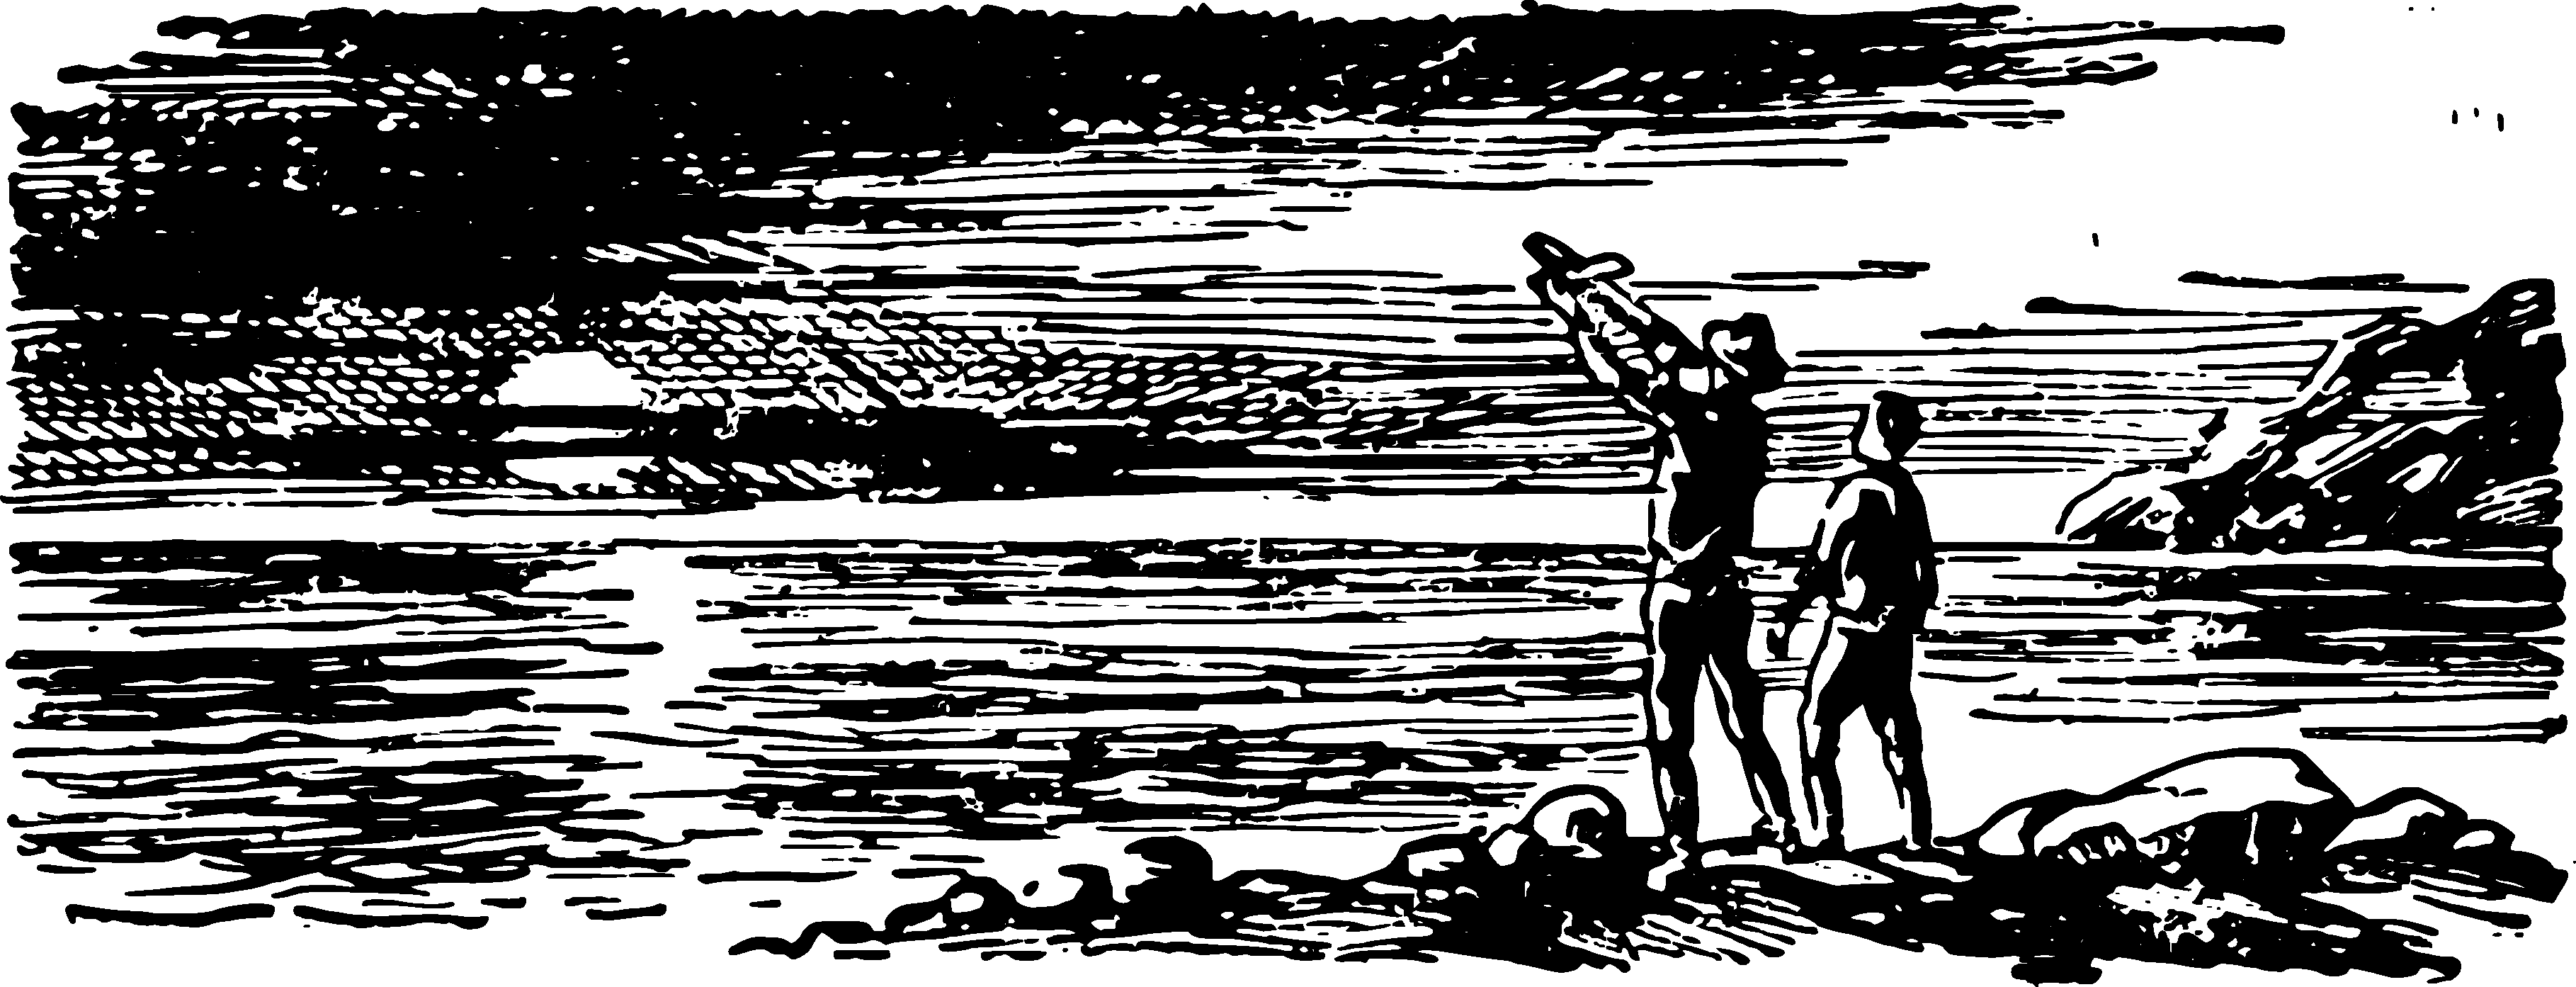
\includegraphics[width=1.2\textwidth]{figures/ch-07/fig-ch-07-head.pdf}\bigskip}

\chapter{The Geometry Of The Robinsons}
\label{ch-07}

\begin{center}
{\large (A few pages from Jules Verne)}
\end{center}

	
\section{The Geometry of the Starry Sky}
\label{sec-7.1}
\begin{quote}
\emph{The abyss has opened, full of stars;\\
To the stars, there is no count, to the abyss, no bottom.}\\
\begin{flushright}
-Lomonosov
\end{flushright}
\end{quote}

There was a time when the author of this book was preparing himself for a somewhat unusual future: a career as a shipwrecked man. In short, I was thinking of becoming a Robinson Crusoe. If that had come to pass, the present book might have been more interestingly compiled than it is now, but perhaps it would not have been written at all. I didn't have to become Robinson, which I don't regret now. However, in my youth, I fervently believed in my calling as Robinson and prepared for it quite seriously. After all, even the most mediocre Robinson must possess many different types of knowledge and skills not required by people of other professions.

What, above all, does a person cast away by shipwreck on a deserted island have to do? Of course, determine the geographical position of their involuntary abode—latitude and longitude. Unfortunately, this is mentioned only briefly in most stories of old and new Robinsons. In the complete edition of the original `Robinson Crusoe,' you'll find just one line about it, and that's in parentheses:

``In the latitude of \ang{9;22} minutes north of the equator\dots{}''

This frustrating brevity drove me to despair when I was stocking up on the information necessary for my imagined future. I was ready to give up on the career of being the sole inhabitant of a deserted island when the secret was revealed to me in Jules Verne's \emph{The Mysterious Island}.

I don't want to disappoint my readers in Robinsons, but I still think it's worth pausing here to discuss the simplest methods of determining geographical latitude. This skill may come in handy not only for the inhabitants of unknown islands. We still have so many inhabited places not marked on maps (and is there always a detailed map at hand?), that the task of determining geographical latitude may arise for many of my readers. True, we cannot assert, like Lermontov once did, that even: ``Tambov is not always marked on the general map by the Circle''; but many villages and collective farms are still not marked on the general maps even today. There's no need to embark on maritime adventures to find yourself in the role of Robinson, for the first time determining the geographical position of your whereabouts.


The matter at hand is fundamentally relatively straightforward. Observing the clear starry sky at night, you will notice that the stars slowly describe inclined circles on the celestial sphere, as if the entire dome of the sky were smoothly rotating around an obliquely positioned invisible axis. In reality, however, you yourself, rotating together with the Earth, describe circles around its axis in the opposite direction. The only point of the starry dome in our northern hemisphere that remains stationary is the one where the imaginary extension of the Earth's axis meets, which is the northern ``pole of the world'' not far from the bright star at the end of the tail of the Little Dipper -- the Pole Star. By locating it in our northern sky, we thereby find the position of the northern pole of the world. Finding it is not difficult if you first locate the position of the well-known constellation Ursa Major: draw a straight line through its extreme stars, as shown in \figr{fig-107}, and, continuing it for a distance approximately equal to the length of the entire constellation, you will arrive at the Pole Star.


\begin{figure}[h!]
\centering
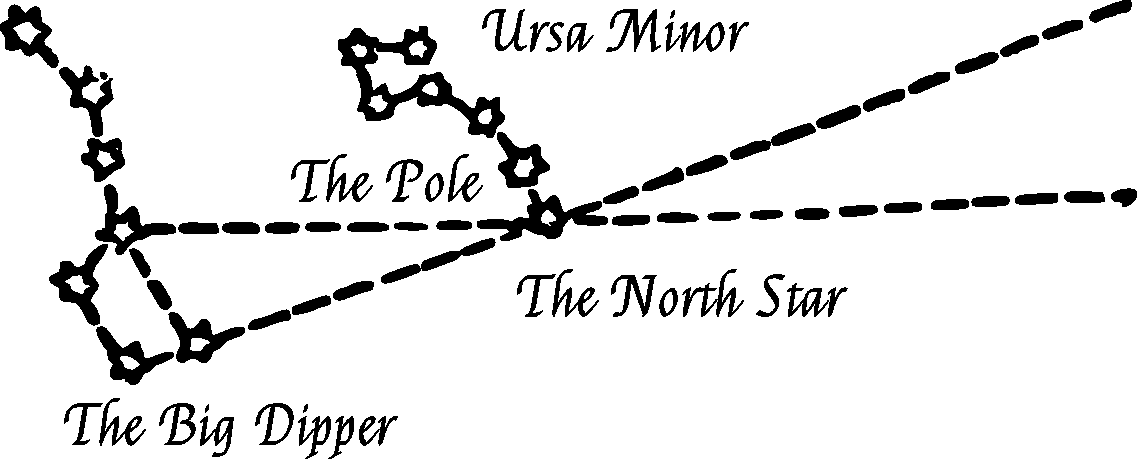
\includegraphics[width=0.8\textwidth]{figures/ch-07/fig-107.pdf}
\sidecaption{The search for the North Star.\label{fig-107}}
\end{figure}



This is one of those points on the celestial sphere that we will need to determine geographical latitude. The second is the so-called ``zenith'', which is the point in the sky directly above your head. In other words, the zenith is the point in the sky where the imaginary extension of the radius of the Earth, which passes through your current location, meets. The degree distance along the celestial arc between your zenith and the Pole Star is at the same time the degree distance of your location from the Earth's pole. If your zenith is \ang{30} away from the Pole Star, then you are \ang{30} away from the Earth's pole, and therefore \ang{60} away from the equator; in other words, you are located on the 60th parallel.

Therefore, to find the latitude of any location, you simply need to measure in degrees (and its fractions) the ``zenith distance'' to the Pole Star; after this, subtract this value from \ang{90} -- and the latitude is determined. Alternatively, you can practically approach it differently. Since the arc between the zenith and the horizon contains \ang{90}, subtracting the zenith distance to the Pole Star from \ang{90} gives us nothing else but the length of the celestial arc from the Pole Star to the horizon; in other words, we obtain the ``altitude'' of the Pole Star above the horizon. Therefore, the geographical latitude of any location is equal to the height of the Pole Star above the horizon of that location.

Now you understand what needs to be done to determine the latitude. Waiting for a clear night, you locate the Pole Star in the sky and measure its angular height above the horizon; the result immediately gives you the sought latitude of your location. If you want to be precise, you should take into account that the Pole Star does not strictly coincide with the pole of the world but is offset from it by \ang{1.25}. Therefore, the Pole Star does not remain completely stationary: it describes a small circle around the stationary celestial pole, moving higher and lower, to the right and left, by \ang{1.25}. By determining the height of the Pole Star in its highest and lowest positions (an astronomer would say: at its upper and lower ``culminations''), you take the average of both measurements. This is the true height of the pole, and consequently, the latitude of the location sought.


But if that's the case, there's no need to choose the Pole Star specifically; you can stop at any non-setting star and, by measuring its height in both extreme positions above the horizon, take the average of these measurements. As a result, you will obtain the height of the pole above the horizon, i.e., the latitude of the location. However, you must be able to catch the moments of the highest and lowest positions of the chosen star, which complicates matters; and it's not always possible to observe this within one night. That's why for the initial approximate measurements, it's better to work with the Pole Star, disregarding its slight deviation from the pole.

Up to now, we've imagined ourselves in the northern hemisphere. How would you proceed if you found yourself in the southern hemisphere? Exactly the same way, with just one difference: here, you need to determine the height of the southern pole instead of the northern pole. Unfortunately, near this pole, there is no bright star like the Pole Star in our hemisphere. The famous Southern Cross shines quite far from the southern pole, and if we want to use the stars of this constellation to determine the latitude, we will have to take the average of two measurements -- at the highest and lowest positions of the star.

The heroes of Jules Verne's novel, \emph{The Mysterious Island}, used precisely this beautiful constellation of the southern sky to determine the latitude of their ``mysterious island''.

It's instructive to reread the passage in the novel where the whole procedure is described. At the same time, we'll learn how the new Robinsons coped with their task without having a sextant.



\section{The latitude of the `Mysterious island'}

It was 8 o'clock in the evening. The moon had not yet risen, but the horizon was already shimmering with delicate pale shades, which could be called lunar dawn. In the zenith, the constellations of the southern hemisphere sparkled, and among them was the Southern Cross. Engineer Smith observed this constellation for some time.

``Herbert,'' he said after some thought, ``is today April 15th?''

``Yes,'' the youth replied.

``If I'm not mistaken, tomorrow is one of those four days in the year when true time equals mean time: tomorrow, the Sun will cross the meridian exactly at noon according to our clocks.\sidenote{Our clocks do not strictly correspond to solar time: there is a discrepancy between ``true solar time'' and the ``mean time'' shown by accurate clocks, which equals zero only four days a year: around April 16th, June 14th, September 1st, and December 24th. (See \emph{Astronomy for Entertainment} by Ya. I. Perelman.)} If the weather is clear, I'll be able to approximately determine the longitude of the island.''

``Without instruments?''

``Yes. The evening is clear, so today I will try to determine the latitude of our island by measuring the height of the stars of the Southern Cross, i.e., the height of the southern pole above the horizon. And tomorrow at noon, I will determine the longitude of the island.''

``If the engineer had had a sextant -- an instrument allowing precise measurement of angular distances between objects using the reflection of light rays -- the task would have been no trouble at all. Having determined the height of the pole that evening, and the next day at noon -- the moment when the Sun passed through the meridian, he would have obtained the geographic coordinates of the island: latitude and longitude. But there was no sextant, so it had to be replaced.''

``The engineer entered the cave. By the light of the campfire, he cut out two rectangular planks, which he connected at one end in the shape of a compass, so that the legs could be shifted and spread apart. For the hinge, he used a strong acacia thorn found among the debris by the campfire.''

``When the instrument was ready, the engineer returned to the shore. He needed to measure the height of the pole above the horizon, clearly defined, i.e., above sea level. For his observations, he went to the platform of the Distant View -- taking into account also the height of the platform above sea level. This last measurement could be done on another day using elementary geometry techniques.''

``The horizon, illuminated from below by the first rays of the moon, was sharply outlined, providing all the conveniences for observation.''

``The constellation of the Southern Cross shone in the sky upside down: the star alpha, indicating its base, lies closer to the South Pole (of the world).''

``This constellation is not located as close to the South Pole as the Pole Star is to the North. The star alpha is \ang{279} away from the pole; the engineer knew this and planned to incorporate this distance into his calculations. He awaited the moment when the star passed through the meridian -- which facilitates the operation.''

``Smith directed one leg of his wooden compass horizontally, the other towards the star alpha of the Cross, and the hole formed by the angle gave the angular height of the star above the horizon. To fix this angle reliably, he nailed a third plank across both planks using acacia thorns, so that the figure maintained its unchanged form.''

``All that remained was to determine the magnitude of the angle obtained, relating the observation to sea level, i.e., taking into account the lowering of the horizon, for which it was necessary to measure the height of the cliff.\sidenote{Since the measurement was taken by the engineer not at sea level but from a high cliff, the line of sight from the observer's eye to the edge of the horizon did not strictly coincide with the perpendicular to the Earth's radius but formed some angle with it. However, this angle was so small that it could be safely neglected for this case (at a height of 100 meters, it barely constitutes a third of a degree; therefore, there was no need for Smith, or rather Jules Verne, to complicate the calculation by introducing this correction.)} The magnitude of the angle would give the height of the star alpha Crucis, and therefore the height of the pole above the horizon, i.e., the geographical latitude of the island, since the latitude of any place on Earth is equal to the height of the pole above the horizon of that place. These calculations were planned to be carried out the next day.''

How the measurement of the height of the cliff was done, my readers already know from the excerpt provided in the first chapter of this book. Skipping this part of the novel here, let's follow the further work of the engineer:

``The engineer took the compass, which he had constructed the day before and with which he had determined the angular distance between the star alpha of the Southern Cross and the horizon. He carefully measured the magnitude of this angle using a circle divided into 360 parts and found that it was equal to \ang{10}. Hence, the height of the pole above the horizon -- after adding \ang{10} to the \ang{27} that separate the named star from the pole, and bringing the height of the cliff, from the top of which the measurement was made, to sea level -- was found to be \ang{37}. Smith concluded that the island of Lincoln was located at \ang{37} South latitude, or -- considering the imperfection of the measurement — between the 35th and 40th parallels.''

All that remained was to find out its longitude. The engineer planned to determine it on the same day, at noon, when the Sun would pass through the meridian of the island.

\section{Determining Geographic Longitude}

``But how will the engineer determine the moment when the Sun crosses the meridian of the island, without having any instruments for it? This question greatly puzzled Herbert.''

``The engineer arranged everything necessary for his astronomical observation. He chose a perfectly clear place on the sandy shore, levelled by the sea tide. A six-foot pole driven into this place was perpendicular to this platform.''

``Herbert then understood how the engineer intended to act to determine the moment of the Sun's passage through the meridian of the island, or, in other words, to determine the local noon. He wanted to determine it by observing the shadow cast by the pole on the sand. This method, of course, is not very accurate, but in the absence of instruments, it still gave quite satisfactory results.

``The moment when the shadow of the object becomes the shortest will be noon. It is enough to carefully monitor the movement of the shadow's tip to notice the moment when the shadow, having stopped decreasing, begins to lengthen again. In this case, the shadow played the role of a clock hand on a dial.''

``When, according to the engineer's calculation, it was time for observation, he knelt down and, driving small stakes into the sand, began to mark the gradual shortening of the shadow cast by the pole.''

``The journalist (one of the engineer's companions) held his chronometer in his hand, preparing to notice the moment when the shadow became the shortest. Since the engineer conducted the observation on April 16, one of those days when true noon coincides with mean noon, the moment observed by the journalist on his chronometer would be established by the time of the Washington meridian (the departure point for the travelers).''

The Sun moved slowly. The shadow gradually shortened. Finally noticing that it began to lengthen, the engineer asked:

`What time is it?'

`Five hours and one minute,' replied the journalist.

``The observation was completed. Only a simple calculation remained to be done.''

``The observation established that the time difference between the Washington meridian and the meridian of Lincoln Island was almost exactly 5 hours. This means that when it is noon on the island, it is already 5 p.m. in Washington. The Sun in its apparent daily motion around the globe covers \ang{1} in 4 minutes, and in an hour, \ang{15}. Thus in one hour it equals $4 \times \ang{15} = \ang{75}$ minutes''

``Washington lies on the meridian \ang{77;53;11} west of the Greenwich meridian, accepted by both Americans and the English as the initial one. This means that the island lay approximately on the 152nd west longitude.''

Taking into account the insufficient accuracy of the observations, it could be asserted that the island lies between the 35th and 40th parallels of south latitude and between the 150th and 155th meridians west of Greenwich.

In conclusion, it should be noted that there are several quite diverse methods for determining geographic longitude. The method used by the characters of Jules Verne is just one of them (known as the `method of carrying chronometers'). Similarly, there are other, more accurate methods for determining latitude than the one described here (not suitable for navigation, for example).


\begin{center}
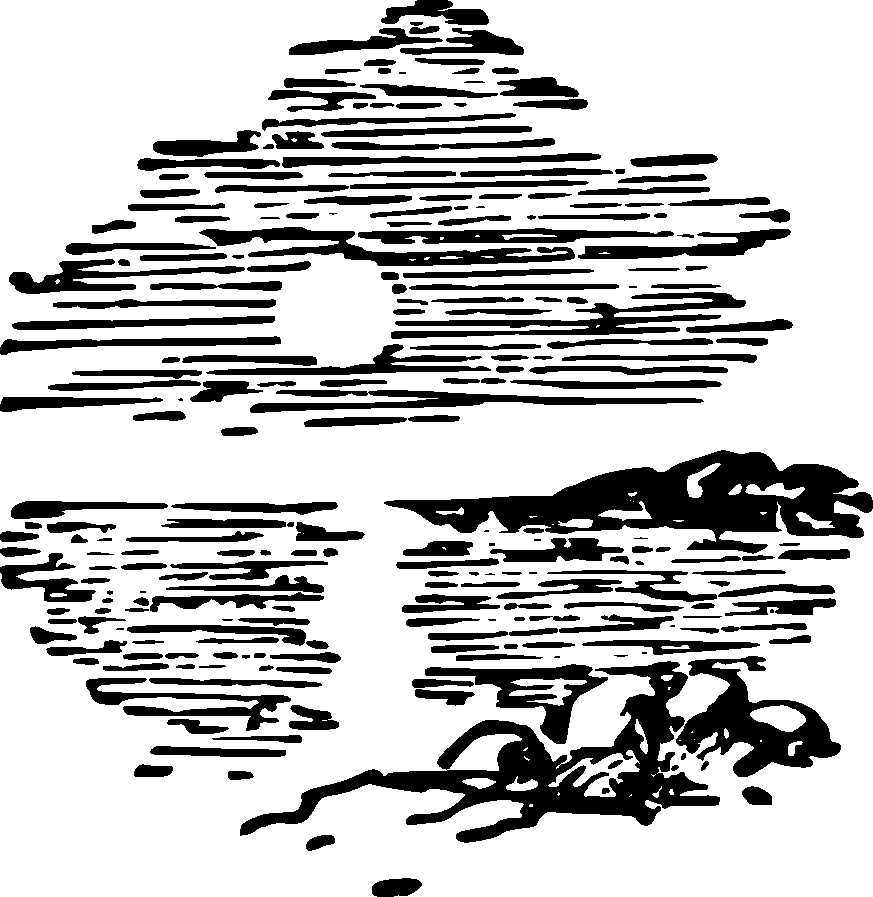
\includegraphics[width=0.3\textwidth]{figures/ch-07/fig-ch-07-tail.pdf}
\end{center}


















